\documentclass[12pt, a4paper]{article}
\usepackage[brazil]{babel}
\usepackage[utf8]{inputenc}
\usepackage[T1]{fontenc}
\usepackage{times}
\usepackage{setspace}
\usepackage[margin=3cm]{geometry}
\usepackage{indentfirst}
\usepackage{graphicx}
\usepackage{hyperref}
\usepackage{subcaption} 
\usepackage{float}
\usepackage{amsmath} 
\usepackage{amssymb}

\onehalfspacing
\setlength{\parindent}{1.5cm}

\newcommand{\titulopt}{Fluxo óptico para análise de calçadas}
\newcommand{\tituloen}{Project Title}
\newcommand{\orientadores}{Roberto Marcondes Cesar Junior \\ Roberto Hirata Junior}
\newcommand{\processo}{ Chamada FAPESP Futuros Cientistas}

\begin{document}

\begin{titlepage}
    \begin{center}
        \large UNIVERSIDADE DE SÃO PAULO\\
        \large INSTITUTO DE MATEMÁTICA E ESTATÍSTICA\\[3cm]


        \textbf{\Large \titulopt}\\[2cm]
        
        
        \textbf{\large Renzo Real Machado Filho}\\[0.5cm]
        \centering \textbf{Orientadores:} \\
        \orientadores \\[3cm]
        
    
        \processo
        \vfill
        
        São Paulo \\ \today
    \end{center}
\end{titlepage}

\section*{Resumo}


\newpage
\tableofcontents
\newpage

\section{Introdução}

\section{Visão Computacional: Algoritmos e Aplicações \cite{szeliski2010}}

\subsection{Processamento de Imagens}

Nesse capítulo, trataremos do conjunto de operações e técnicas aplicadas a imagens digitais. É uma etapa de preparação para muitos algoritmos de reconhecimento de objetos, reconstrução 3D e/ou rastreamento de movimento. Nessa perspectiva, começaremos pelos chamados "operadores de ponto", que manipulam cada pixel de uma imagem, independentemente daqueles ao seu redor. Depois, passaremos pelos operadores "area-based", nos quais cada novo valor de um pixel depende de um certo número de pontos vizinhos.

Um operador genérico é uma função que toma uma ou mais imagens como inputs e produz uma outra imagem de output. Matematicamente,
\[
f(x) = h(g_0(x), \dots, g_n(x))
\]

Já uma imagem digital colorida é representado como uma matriz 3D (altura $\times$ largura $\times$ 3 canais). Os 3 canais são: Blue, Green, Red (em OpenCV é BGR).

\subsection{Operadores de Ponto}

\subsubsection{Transformações de Pixels}

\noindent\textbf{Ajuste de Brilho (Brightness) e Contraste (Contrast)} \\

\noindent\textbf{Tipo:} Transformação linear.

\noindent\textbf{Fórmula:} $ f(x) = a(x) \cdot g(x) + b(x) $, onde $a$ é dito o contraste e $b$, o brilho.

\noindent\textbf{Efeito:} O brilho desloca uniformemente todos os valores de pixel na imagem. Valores positivos clareiam a imagem, valores negativos escurecem. Enquanto isso, o contraste controla a diferença entre tons claros e escuros. Valores $> 1$ expandem a faixa tonal (aumentam o contraste), valores entre 0 e 1 comprimem a faixa tonal (reduzem o contraste).

\noindent\textbf{Quando usar:} Quando a imagem está muito escura ou muito clara globalmente ou quando a imagem está "chapada", i.e, sem muita variação tonal. \\

\noindent\textbf{Correção Gamma} \\

\noindent\textbf{Tipo:} Transformação não-linear.

\noindent\textbf{Fórmula:} $f(x) = g(x)^{1/\gamma}$.

\noindent\textbf{O que é Gamma ($\gamma$)?} É um parâmetro que define a curvatura da transformação não-linear aplicada aos valores de intensidade. Ele controla como os valores intermediários (tons médios) são mapeados, enquanto preserva os extremos (preto puro e branco puro). Por padrão, usa-se $\gamma \approx 2.2$.

\noindent\textbf{Efeito:} Se $\gamma > 1$, escurece os tons médios enquanto preserva pretos e brancos (aumenta contraste em tons escuros). Já $\gamma < 1$, clareia os tons médios enquanto preserva pretos e brancos (aumenta contraste em tons claros).

\noindent\textbf{Quando usar:} Para corrigir percepção visual ou problemas de iluminação não-lineares. \\

\noindent \textbf{Ordem das Operações} \\

Contraste/Brilho $\rightarrow$ Gamma

O Contraste/Brilho são lineares, trabalham no domínio da intensidade enquanto o Gamma é não-linear, trabalha no domínio perceptual. Se fizéssemos gamma primeiro a transformação linear posterior distorceria a curva gamma e os valores seriam re-escalados de forma inadequada, perdendo o controle preciso sobre a correção tonal.

\subsubsection{Color Balance}
Esse procedimento ajusta a intensidade relativa das cores primárias. A operação é feita por canal (R, G, B). Podemos multiplicá-los por um fator que altera seu brilho ou ainda operar sobre transformações mais complexas, como o mapeamento no espaço de cores XYZ. \\

\noindent\textbf{Espaço de Cores XYZ}\\

É um espaço de cor matematicamente definido, usando coordenadas tridimensionais (X, Y, Z) para descrever todas as cores visíveis ao olho humano.
\begin{itemize}
    \item \textbf{X:} Representa aproximadamente a sensibilidade ao vermelho
    \item \textbf{Y:} Representa o brilho luminoso (luminância)
    \item \textbf{Z:} Representa aproximadamente a sensibilidade ao azul
\end{itemize}

\subsubsection{Composição e Mascaramento (Compositing and Matting)}

Em muitos aplicativos de edição de fotos e de efeitos visuais, queremos inserir/combinar elementos em uma imagem. Esse processo é chamado de \textbf{composição} \cite{SmithAndBlinn:1996:BSM}.

Paralelo a isso, também é desejável extrair objetos de imagens, processo comumente chamado de \textbf{mascaramento}. Uma máscara define a área de uma imagem que deve ser mantida ou ignorada, permitindo que apenas certas partes da imagem sejam visíveis e sejam integradas com outros elementos \cite{Porter:1984:CDI, SmithAndBlinn:1996:BSM}. \\

\noindent \textbf{Alpha matting} \\

É um processo que visa estimar a translucidez de um objeto em uma determinada imagem. O "alpha matting" resultante descreve, em pixels, a quantidade de cores de primeiro e segundo plano que contribuem para a cor da imagem composta. \cite{germer2020fastmultilevelforegroundestimation} \\

\noindent \textbf{Alpha-Matted Color Image} \\

É uma imagem que além dos 3 canais de cor (RGB), possui um 4º canal intermediário (Alpha - $\alpha$) que representa:
\begin{itemize}
    \item $\alpha = 1$: Pixel totalmente opaco
    \item $\alpha = 0$: Pixel totalmente transparente
    \item $0 < \alpha < 1$: Pixel parcialmente transparente
\end{itemize}

Portanto, para compor uma nova imagem sobre uma imagem antiga, o \textit{over operator} é

\[
C = (1-\alpha) B + \alpha F
\]

A equação acima atenua a influência da imagem de fundo $B$ por um fator $(1 - \alpha)$ e,
em seguida, adiciona os valores de cor (e opacidade) correspondentes à camada de primeiro plano $F$.

\subsubsection{Equalização de Histograma}

O histograma de uma imagem é um gráfico que representa a frequência de cada nível de intensidade de cinza (ou cor) presente na imagem. Em uma imagem de 8 bits em escala de cinza, por exemplo, existem 256 níveis de intensidade, que vão de 0 (preto absoluto) a 255 (branco absoluto). O eixo horizontal do histograma representa esses níveis de intensidade, enquanto o eixo vertical indica o número de pixels que possuem cada uma dessas intensidades.

Imagens com baixo contraste tendem a ter seus histogramas concentrados em uma faixa estreita de valores. Por exemplo, uma imagem escura terá a maioria de seus pixels com valores de intensidade baixos, resultando em um histograma "amontoado" à esquerda. De forma análoga, uma imagem muito clara terá seu histograma concentrado à direita.

\begin{figure}[H]
    \centering
    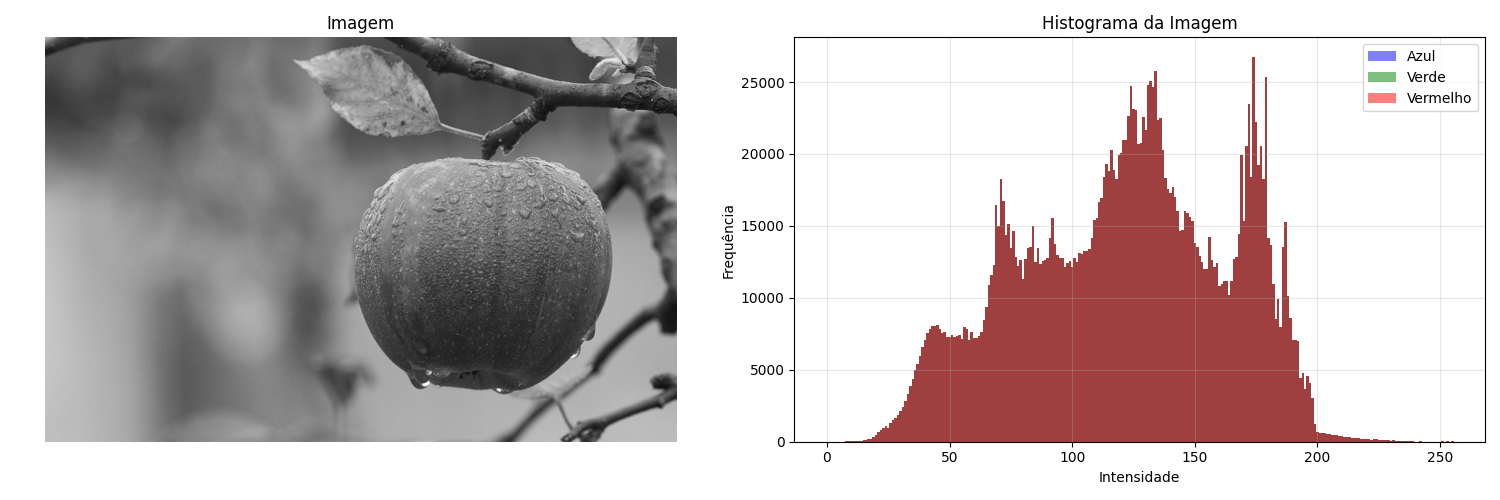
\includegraphics[width=1\linewidth]{Images/img+hist.png}
\end{figure}

\begin{figure}[H]
    \centering
    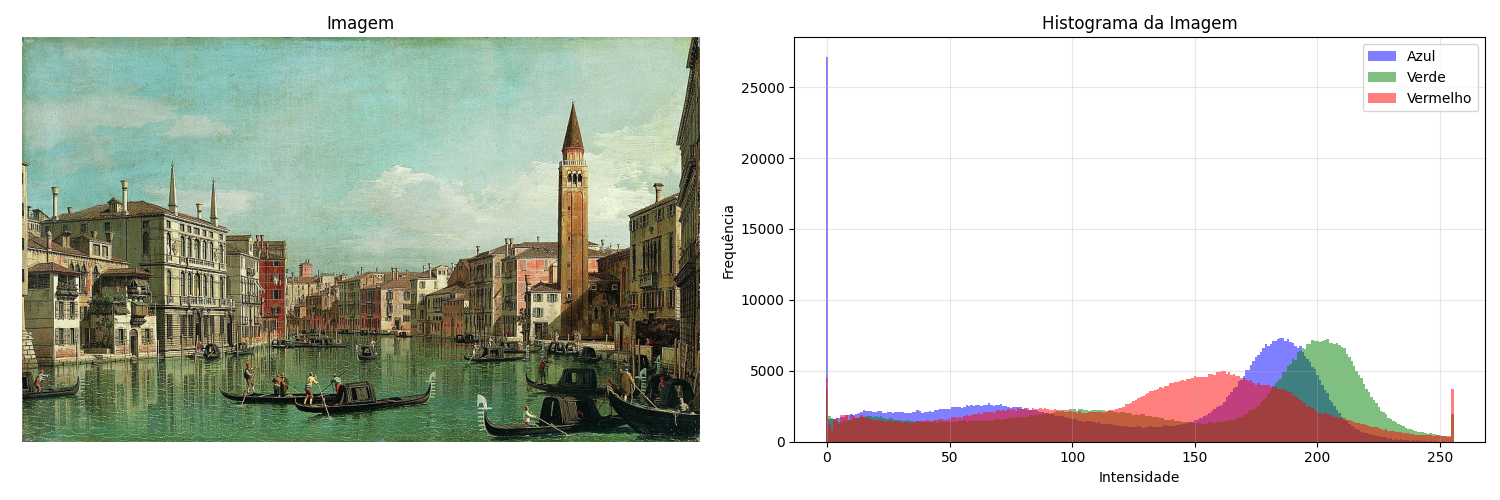
\includegraphics[width=1\linewidth]{Images/img+hist2.png}
\end{figure}

A equalização de histograma atua justamente nesse cenário, redistribuindo igualmente esses valores de intensidade por toda a gama possível. O objetivo é transformar o histograma original em um histograma mais próximo de uma distribuição uniforme, onde cada nível de intensidade tenha, idealmente, o mesmo número de pixels. Ao fazer isso, a diferença de intensidade entre os pixels é acentuada, o que melhora significativamente o contraste global da imagem.

Para isso, computamos a Função de Distribuição Acumulada (CDF), denotada por $c(I)$

\[
c(I) = \frac{1}{N}\sum_{i=0}^I h(i) = c(I-1) + \frac{1}{N}h(I),
\]

\noindent onde $I$ é o nível de intensidade atual (0-255 para imagens 8-bit), $h(I)$ é a frequência do nível de intensidade $I$ (valor do histograma) e $N$ é quantidade de pixels na imagem.

\section{Fluxo Óptico}

O fluxo óptico é definido como a distribuição das velocidades aparentes do movimento dos padrões de brilho em uma imagem. \cite{Horn1981}. 

\subsection{Campo de Movimento (Motion Field)}

Trata-se da velocidade de um ponto que se move na cena/imagem. Em muitos casos, esse conceito se confunde com o fluxo óptico. 

\subsection{\textit{Optical Flow Constraint Equation}}

Suponha que temos um ponto $(x,y)$ numa imagem que se moveu para $(x+\delta x, y+\delta y)$. O seu  deslocamento é $(\delta x, \delta y)$ e queremos medir esse movimento. Dizemos que o fluxo óptico é $(u, v) = (\frac{\delta x}{\delta t}, \frac{\delta y}{\delta t})$ num tempo $\delta t$, pequeno. \\

\textit{Suposição 1:} O brilho de um ponto é constante ao longo do tempo. Então, 

\[ I(x, y, t) = I(x+ \delta x, y + \delta y, t+\delta t).\]

\textit{Suposição 2:} O deslocamento $(\delta x, \delta y)$ e o passo $\delta t$ são pequenos. \\

Com isso, por Taylor, temos

\[ f(x+\delta x) = f(x) + \frac{\partial f}{\partial x} \delta x + \dots + \frac{\partial^n f}{\partial x^n} \frac{\delta x^n}{n!}\]

Se $\delta x \to \infty$, então $f(x + \delta x) = f(x) + \frac{\partial f}{\partial x} \delta x + O(\delta x^2)$.

Para $\delta x, \delta y$ e $\delta t$ suficientemente pequenos, vale que

\[ f(x + \delta x, y + \delta y, t + \delta t) \approx f(x, y, t) + \frac{\partial f}{\partial x} \delta x + \frac{\partial f}{\partial y} \delta y + \frac{\partial f}{\partial t} \delta t \]

Pela \textit{suposição 2}, temos

\[ I(x + \delta x, y + \delta y, t + \delta t) = I(x, y, t) + I_x \delta x + I_y \delta y + I_t \delta t\]

Pela \textit{suposição 1} e subtraindo ambas as equações, obtemos

\[ I_x \delta x + I_y \delta y + I_t \delta t = 0\]

Dividindo por $\delta t$ e com $\delta t \to 0$, temos

\[ I_x \frac{\delta x}{\delta t} + I_y \frac{\delta y}{\delta t} + I_t  = 0\]
\[ \Leftrightarrow I_x u + I_y v + I_t  = 0, \]

onde $(u, v)$ é o fluxo óptico.

\subsubsection{Problema da Abertura}

\subsection{O método de Lucas-Kanade}

Vimos que, pelo resultado anterior, a equação de restrição de fluxo óptico é um problema mal posto. Assim, é necessário mais uma suposição. \\

\textit{Suposição 3:} para cada pixel, assuma que o campo de movimento e o fluxo óptico são constantes em uma pequena vizinhança $W$.

Para quaisquer $(l,k) \in W$, vale

\[ I_x(l,k) u + I_y(l,k) v + I_t(l,k)  = 0 \]

Isso resulta em um sistema de equações. Logo, na forma matricial para $W_{n\times n}$, temos

\[
\underbrace{
\begin{bmatrix}
I_x(1,1) & I_y(1,1) \\
\vdots & \vdots \\
I_x(n,n) & I_y(n,n)
\end{bmatrix}
}_{A}
\underbrace{
\begin{bmatrix}
u \\
v
\end{bmatrix}
}_{x}
=
\underbrace{
\begin{bmatrix}
I_t(1,1) \\
\vdots \\
I_t(n,n)
\end{bmatrix}
}_{B}
\]

Esse é um clássico problema do tipo $Ax=B$. Portanto, podemos resolvê-lo por mínimos quadrados, obtendo

\[
x = (A^T A)^{-1}A^TB.
\]

\subsubsection{Condições}

\begin{itemize}
    \item $A^TA$ deve ser inversível
    \item $A^TA$ deve estar bem condicionada:
    \begin{itemize}
        \item Sejam $\lambda_1, \lambda_2$ os autovalores de $A^TA$. Então, $|\frac{\lambda_1}{\lambda_2}| \approx 1$ e $\lambda_1, \lambda_2 > \epsilon$.
    \end{itemize}
\end{itemize}

As seguintes situações descrevem situações comuns: \\

\textbf{Regiões Homogêneas}

Regiões sem muita textura dificultam a visualização de movimento. Matematicamente, $\lambda_1 \approx \lambda_2$, mas ambos são pequenos. \\

\textbf{Bordas}

Regiões com presença de bordas geram um problema mal condicionado. Os gradientes estão predominantemente em um direção, i.e, a variação significativa está em uma única direção. Assim, o resultado da estimação de fluxo óptico pode ser ambíguo. Matematicamente, $\lambda_1 >>> \lambda_2$. \\

\textbf{Regiões Texturizadas}

Nesse cenário, a estimativa é muito boa. Há muitas variações nos padrões de brilho. Matematicamente, $\lambda_1 \approx \lambda_2$ e $\lambda_1, \lambda_2 > \epsilon$.

\subsection{Coarse-To-Fine Flow Estimation (Estimação de Fluxo do "Grosso ao Fino") }

Quando temos uma sequência de imagens com grandes movimentos, a aproximação por série de Taylor não é mais válida, bem como suas suposições.


\section{State-of-Art}

A estimação de movimento nas cenas pode ser dividido em três métodos: knowledge-driven, data-driven e hybrid-driven. 

\subsection{knowledge-driven}

É baseado em suposições para restringir o processo de estimação e modelar a correspondência espacial-temporal. Os primeiros métodos são Horn e Schunck (HS) e Lucas e Kanade (LK). 

\subsection{Desafios}

\subsubsection{Grandes Deslocamentos}

Objetos que se movem em rapidamente producem grandes distâncias entre os pixels nas cenas, o que dificulta o cálculo. Para lidar com esse problema, é usual utilizar uma estratégia "fino ao grosso" (coarse-to-fine).

\subsubsection{Oclusão}

A oclusão é o processo de detectar e/ou rastrear objetos quando estão ocultos ou obstruídos numa cena. Os métodos mais comuns adotam um esquema de verificação de consistência.

\subsubsection{Variações de Iluminação}

A clássica suposição de constância do brilho não se aplica em contextos de mudanças de iluminação. ???

\subsubsection{Ruído}

Filtros são aplicados em um campo para reduzir o ruído e melhorar a qualidade do mapeamento do fluxo.

\subsection{Data-driven}

As técnicas mais dominantes utilizam o deep learning. As CNNs tem sido muito bem sucedidas para a estimação de fluxo óptico. Por sua vez, esses métodos se divivem em U-Net e em Rede de Pirâmide Espacial.

\subsubsection{U-Net}

Utiliza a estrutura de encoder-decoder. Por causa da contração e expansão do mapeamento de features nos encoders e decoders, há perda de detalhes importantes, o que é prejudicial para a estimação densa de movimento e atrapalha a acurácia e o detalhamento do campo de fluxo.

\section{Escala de Cinza}
O Cálculo da Escala de Cinza

Seu raciocínio de usar a média (R+G+B)/3 é perfeitamente lógico e seria a forma mais simples de fazer a conversão. No entanto, o método padrão é um pouco mais complexo, e o motivo é fascinante: a biologia do olho humano!

Nossos olhos não são igualmente sensíveis a todas as cores. Somos muito mais sensíveis à luz verde, um pouco menos à vermelha e bem menos à azul.

Para criar uma representação em escala de cinza que pareça "natural" para um ser humano em termos de brilho percebido, a conversão usa uma média ponderada. Os canais de cor que percebemos melhor têm um peso maior no cálculo final.

A fórmula padrão (usada pelo OpenCV e em muitas outras aplicações) é:

Y=0.299⋅R+0.587⋅G+0.114⋅B

Onde Y é o valor do pixel de luminância (o valor de cinza).

Veja como o Verde (G) tem um peso enorme (quase $60\%$), enquanto o Azul (B) tem um peso bem pequeno. Isso garante que uma imagem com muito verde pareça mais clara em escala de cinza do que uma imagem com muito azul, o que corresponde à nossa percepção.

\bibliographystyle{IEEEtran}
\bibliography{refs}

\end{document}